\documentclass{lposter}
\usepackage{graphicx}
\usepackage{natbib}
\usepackage{booktabs}
\usepackage{subfigure}
\usepackage{amsmath}
\usepackage{algpseudocode}
\usepackage{alltt}
\usepackage{textcomp}
\usepackage{url}
\usepackage{amssymb, amsthm, bm}
%\usepackage{semantic}
\usepackage{eso-pic}

\newcommand\BackgroundPicture{%
\put(0,0){%
\parbox[b][\paperheight]{\paperwidth}{%

\includegraphics[width=\paperwidth,height=\paperheight,%
                   keepaspectratio]{BUCS}%
\vfill%
}}}

\AddToShipoutPicture{\BackgroundPicture}
\bibliographystyle{alpha}

\theoremstyle{plain}
\newtheorem{theorem}{Theorem}
\newtheorem{lemma}{Lemma}
\newtheorem{prop}{Proposition}
\newtheorem{rem}{Remark}
\newtheorem{cor}{Corollary}

\theoremstyle{definition}
\newtheorem{definition}{Definition}
\newtheorem{ex}{Example}

\newcommand{\Z}{\mathbb{Z}}
\newcommand{\N}{\mathbb{N}}
\newcommand{\F}{\mathbb{F}}
\newcommand{\R}{\mathbb{R}}
\newcommand{\C}{\mathbb{C}}
\newcommand{\Q}{\mathbb{Q}}
\newcommand{\E}{\mathbb{E}}
\newcommand{\OC}{\mathcal{O}}
\newcommand{\bi}{\textbf{i}}

\renewcommand{\tt}[1]{\texttt{#1}}
\newcommand{\tts}[1]{\tiny{\texttt{#1}}}
\newenvironment{myprogramtext}
{\begin{list}{}{\setlength{\leftmargin}{1em}}\item\small\bfseries}
{\end{list}}

\department{Computer Science}
\author{Sean Smith UROP advisor Richard West}
\year{2015} \class{} \advisor{Richard West}
\title{Designing an Autonomous Quadcopter}

\providecommand{\bibtex}{{\rmfamily B\kern-.05em%
    \textsc{i\kern-.025em b}\kern-.08em%
    T\kern-.1667em\lower.7ex\hbox{E}\kern-.125emX}}

\pagestyle{fancy}

\begin{document}
\begin{poster}

%Abstract
%Problem
%Significance
%Approach
%results/observations


\section{Quadcopter Characteristics}

\begin{itemize}
\item Uses 6 directional sonar sensors to navigate indoors
\item Will run a version of SLAM called orthoslam that locates planes(walls indoors) and navigates based on a map of the surrounding planes
\item Has four brushless motors that can lift 290 grams so it can lift a total of 775 grams counting the frame and electronics
\item Has a flight time of 12 minutes on a 1300mah battery
\end{itemize}

\section{Motivation}

\begin{itemize}
\item Improvements in hardware and battery technology make it feasible for the first time to fly for extended periods of time in small spaces.
\item The algorithms and software needed to fly indoors largely doesn't exist as most autonomous flight is guided by a human or guided by satellites which do not work indoors
\item We are on the cutting edge of research into autonomous indoor flight and it will be largely done in approximately 5 years.  

\end{itemize}

\section{Build}

\begin{figure}
\centering
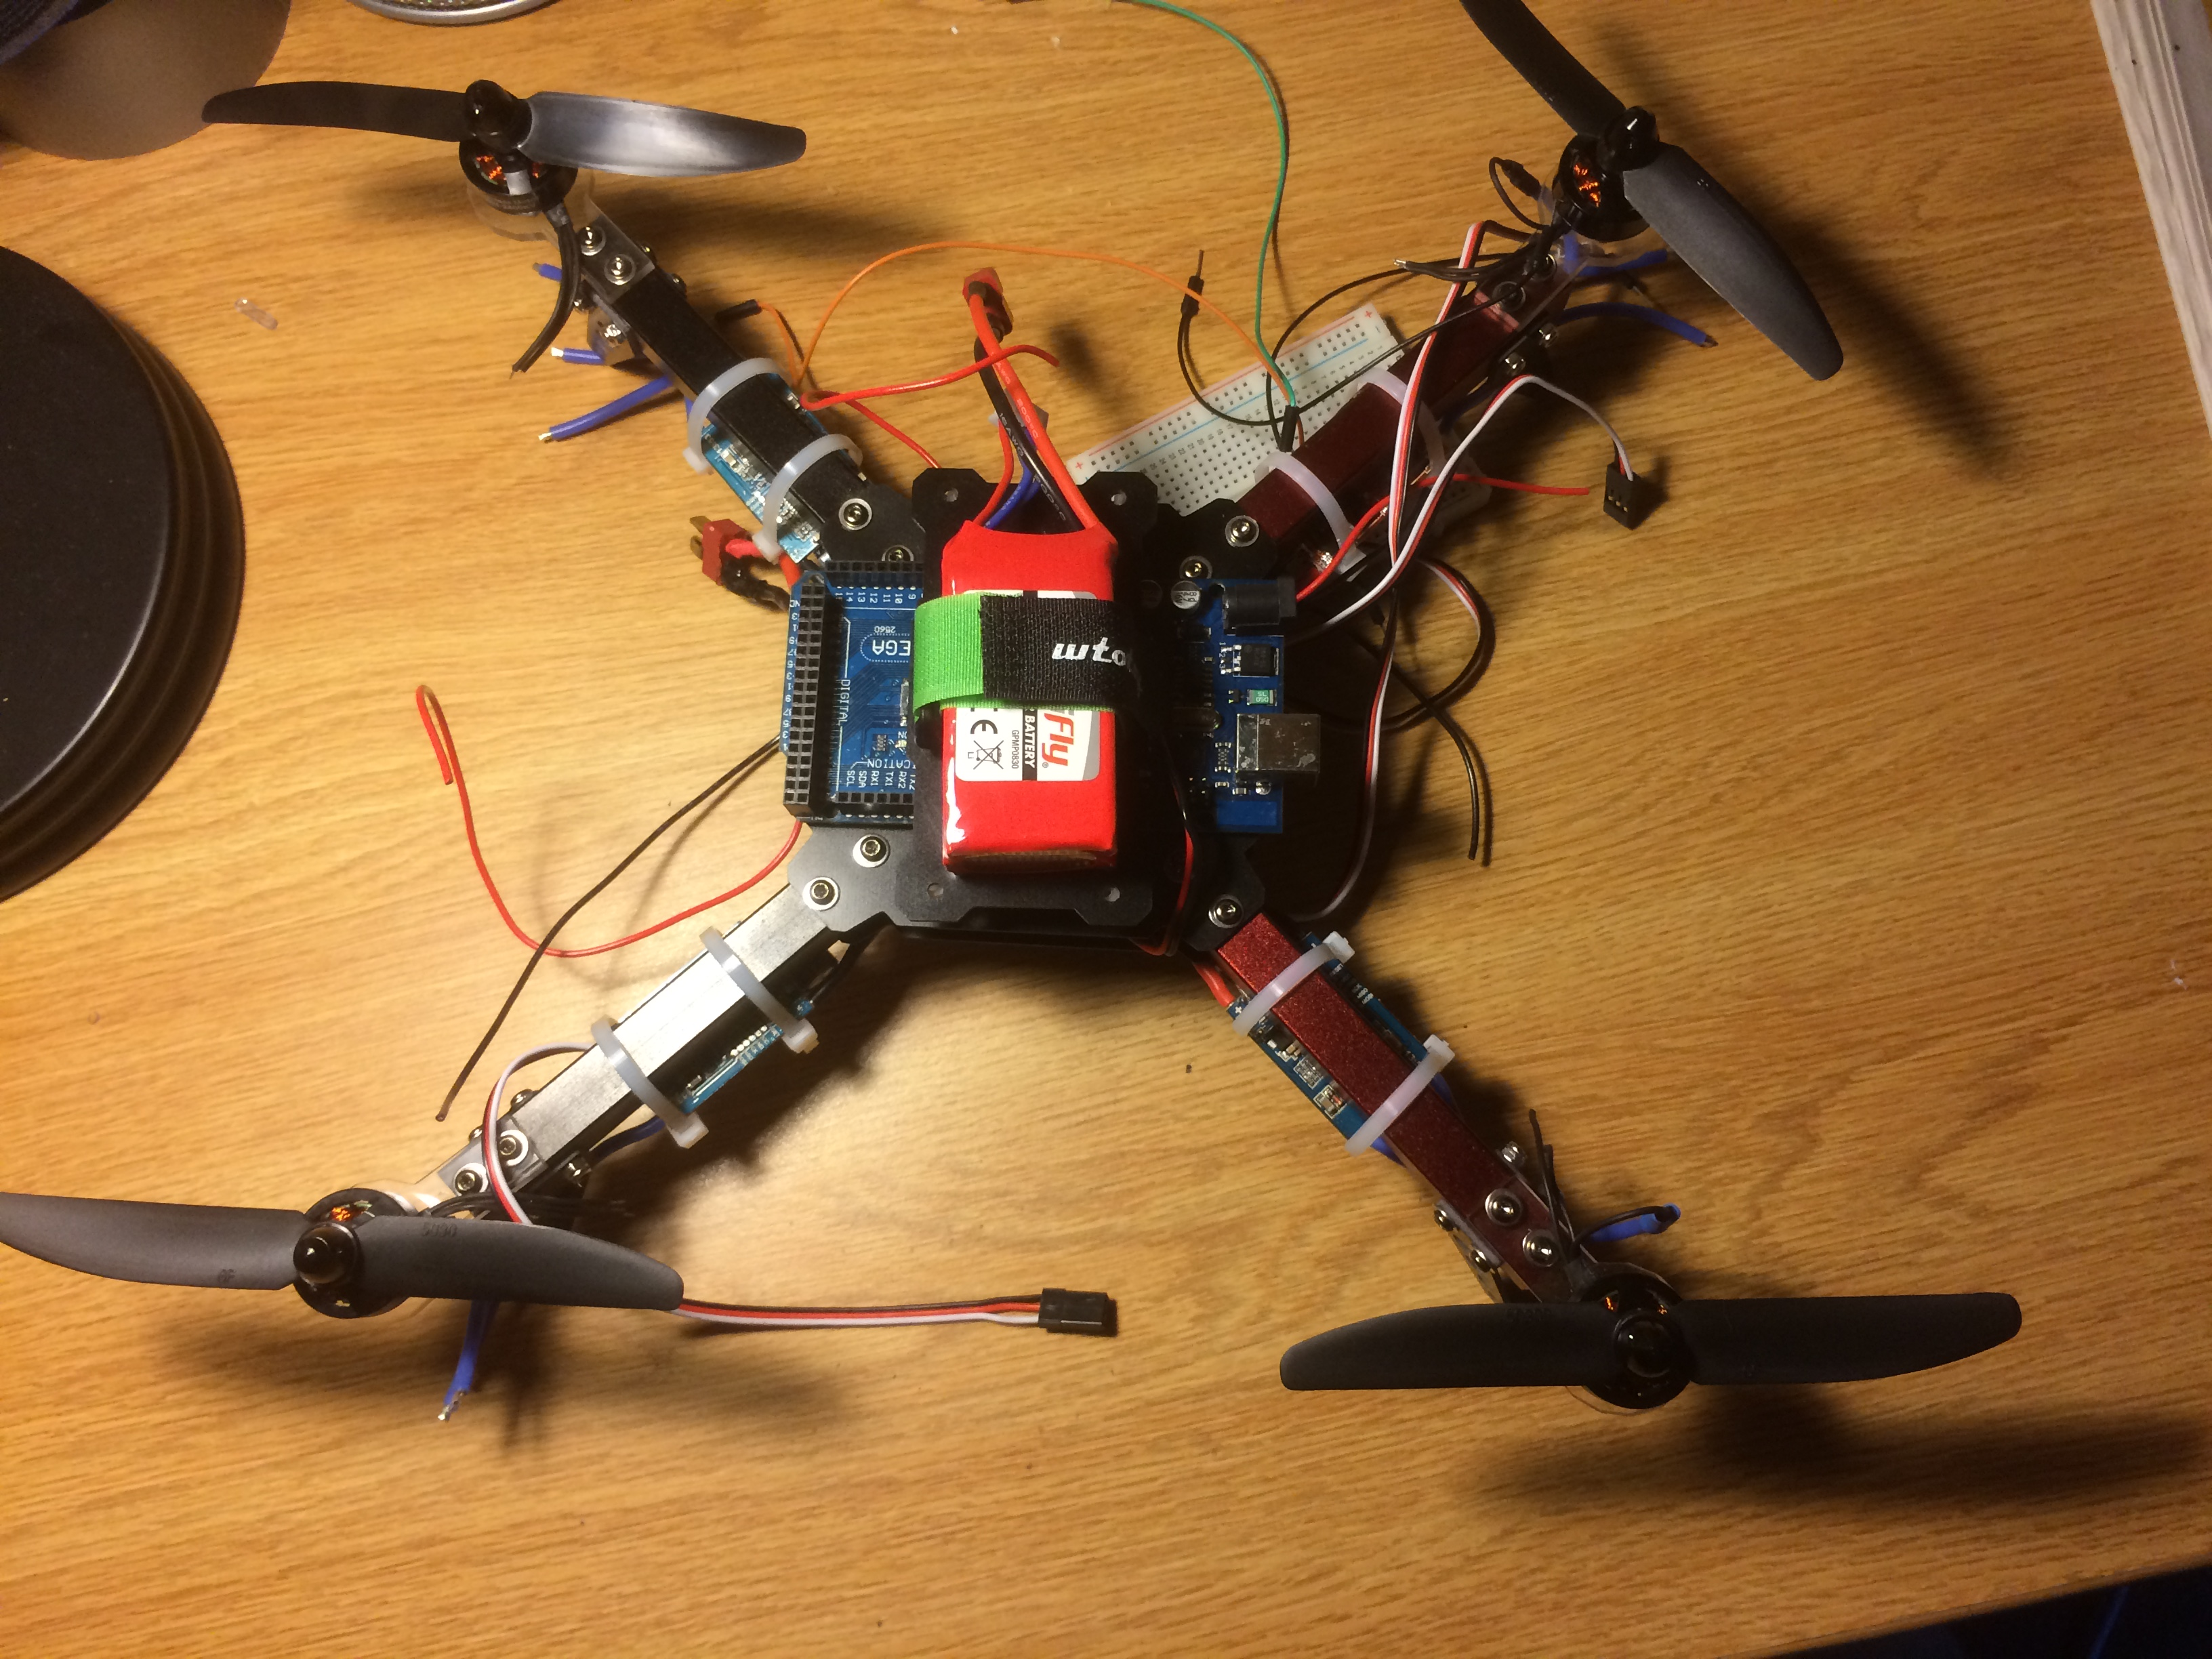
\includegraphics[scale=0.2]{quad.jpg}
\caption{Completed Quadcopter\newline}
\label{fig:mig_over}
\end{figure}

\begin{itemize}
\item Built out of Aluminum and Glass Fiber. The light materials contribute to a low overall weight of 385 grams.
\item Custom designed motor mounts made out of PMMA plastic


%\begin{figure}
%\centering
%\includegraphics[scale=0.5]{mount}
%\caption{Motor Mount\newline}
%\label{fig:mig_over}
%\end{figure}

\item The quadcopter is 10"x10" and fills a space of 15"x15" when the spinning propellors are factored in. Its small size makes in maneuverable in doorways and hallways. 
\end{itemize}


\section{Control Sequence}


\begin{figure}
\centering
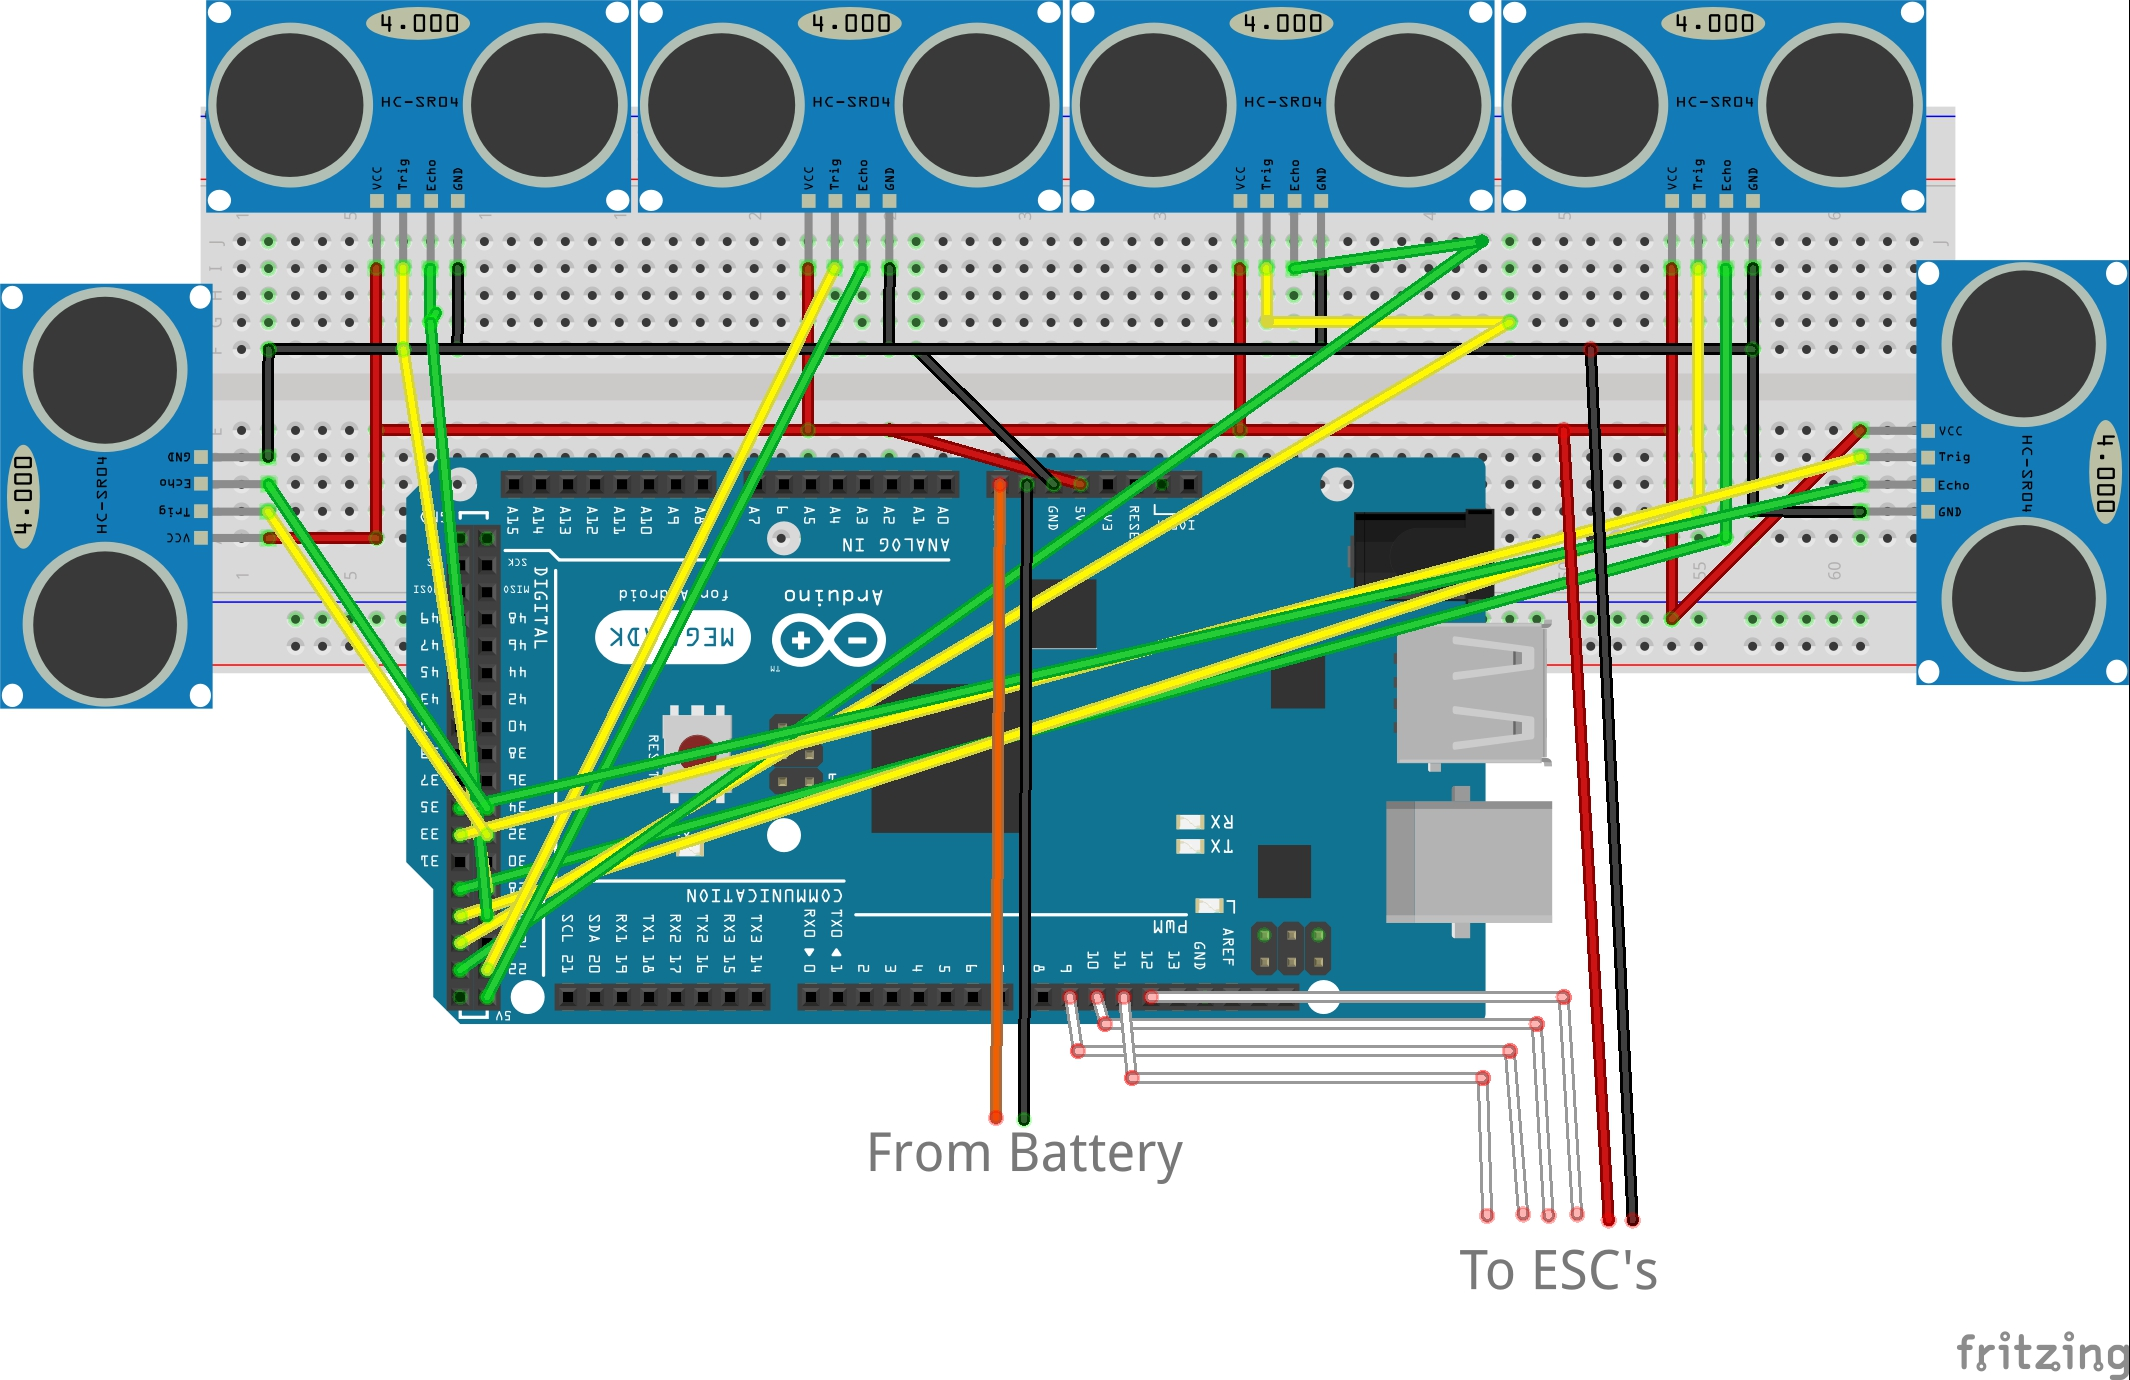
\includegraphics[scale=.9]{quad_fr.jpg}
\caption{Wiring Schematic\newline}
\label{fig:mig_over}
\end{figure}



\begin{itemize}
\item A KK2 Board runs through the PID loop while an Arduino Mega does the Sonar calculations
\item Abstracting the control loop out onto its own board mitigates the overhead causes by running a PID loop as well as checking six sonar inputs
\item The sonar loop is very simple, it first gets to a stable hover at $\approx 5$cm. Then it enters into the navigation loop.
\item The navigation loop runs the difference algorithm and sends it the KK2 board.

\begin{itemize}
\item Takes the path array $h$
\item $i$ is the waypoint counter (initialized to zero)
\item Find the current waypoint $h[i]$
\item $w$ is the current sonar input
\item $r$ is the range of the controller (0-90 for most controllers)
\item Sets $o$ to the square of the difference between $h[i]$ and $w$ divided by $r$

$$ o = \frac{(w - h[i])^2}{r}$$

\end{itemize}

%Navigation Algorithm
\begin{algorithmic}
\Function{main}{$h$}
\State $stableHover()$
\State $flying\gets true$
\State $i\gets 0$
\While{$flying$}
\State $w \gets getSonarInput()$
\State $o \gets \frac{(w - h[i])^2}{r}$
\State $flying \gets sendDifference(o)$
\EndWhile

\EndFunction
\end{algorithmic}

\begin{figure}
\centering
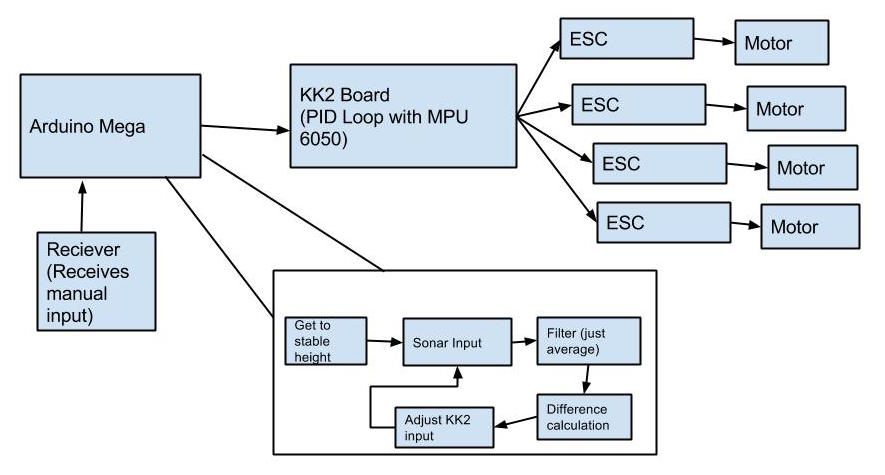
\includegraphics[scale=.8]{quad_state_machine.jpg}
\caption{System Architecture\newline}
\label{fig:mig_over}
\end{figure}


\begin{figure}
\centering
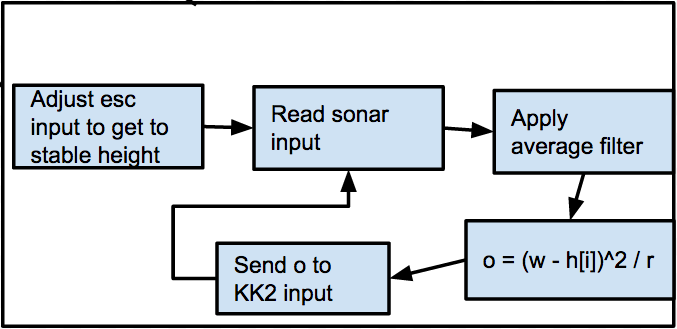
\includegraphics[scale=.8]{code}
\caption{Code Architecture\newline}
\label{fig:mig_over}
\end{figure}
\end{itemize}

\section{Significance}

\begin{itemize}
\item Since the drone can fly in tight spaces with no outside input it makes sense as a mapping tool or data collection platform for situations that put humans at risk
\item This can be used in situations that put humans at risk.
\item In the future this will run on Rich West's Quest operating system.
\end{itemize}

\noindent{\bf Project Website:}~ {\it http://cs-people.bu.edu/swsmith/iap15.pdf}\\
{\bf Quest Website:}~ {\it http://www.questos.org}

\bibliography{iap13}

\end{poster}
\end{document}

